\section{Challenges in MANETs}
\label{sec::challenges}

\begin{figure*}[htb!] 
  \hfill
  \begin{minipage}[t]{.47\textwidth}
    \begin{center}  
      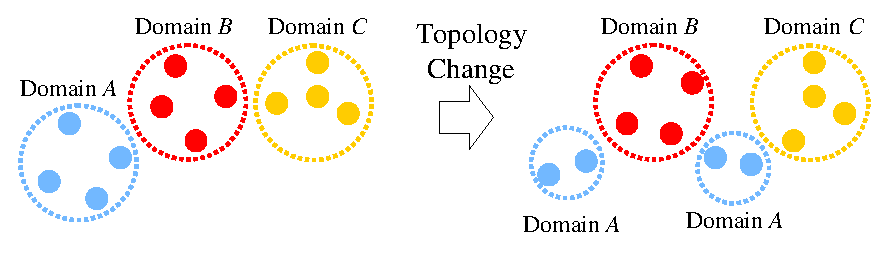
\includegraphics[scale=0.55]{challenges1}
        \caption{The MANET of domain $A$ is partitioned due to mobility.} \label{fig:challenges1}
    \end{center}
  \end{minipage}
  \hfill \quad
  \begin{minipage}[t]{.47\textwidth}
    \begin{center}  
       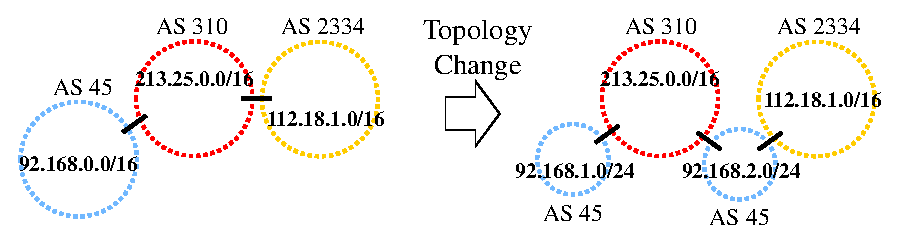
\includegraphics[scale=0.55]{challenges2} 
        \caption{A similar setting in terms of topology change in BGP.} \label{fig:challenges2} 
    \end{center}
  \end{minipage}
  \hfill 
\end{figure*}


MANETs are fundamentally different from wired networks, and the
operating environments of mobile wireless devices have resulted in a
set of new heterogeneous elements to be considered in inter-domain
routing.  One major challenge to provide inter-domain routing to
MANETs is the dynamic nature of network topology. Unlike the Internet,
there are no designate network borders between MANETs because they can
move around to connect via different gateways, and multiple networks
may even geographically overlap some times.

Also, a domain of MANET can be partitioned into disjoint networks
without direct intra-domain connectivity, and the intra-domain
connectivity may only be maintained by traversing the nodes in other
domains. These properties impair the direct application of a
traditional inter-domain routing protocol to MANETs. 
%Next, we illustrate the undesirable impacts of network partition on inter-domain routing.

Consider Figure~\ref{fig:challenges1} consisting of three MANET
domains. One might apply BGP to this scenario as in
Figure~\ref{fig:challenges2}. However, there are several issues that
make BGP inapplicable. First, the path vector protocol in the BGP
implicitly assumes the availability of the following functions:

%\vspace{4pt}

(1) {\bf Internal Gateway Detection:} The internal gateways within
the same domain can detect the presence of each other so that they
know whom to communicate with about the information of external
routes.

%\vspace{4pt}

(2) {\bf Internal Network Knowledge:} The gateways know the
reachable destinations and the internal routes to the destinations
within the domain.

%\vspace{4pt}

These functions are normally supported by the proactive intra-domain
routing protocols (e.g., distance-vector and link-state routing
protocols) through continual maintenance of network state information.
However, we cannot always assume the availability of this information
in MANETs that uses a reactive routing protocol in their
domains, as they do not necessarily provide these functions out of
their regular operation. Without careful design, a direct application
of a path vector protocol over MANETs with add-on processes to support
these functions may be undesirable to MANETs with dynamic node
mobility and scarce wireless communication bandwidth.


Second, in BGP every destination is identified by an IP address, which
follows a certain network hierarchy. To announce the destinations in a
domain, gateways will aggregate the IP addresses in the domain by
suitable IP prefixes (e.g., 92.168.0.0/16).  However, in MANETs,
mobility and ad hoc deployment can create arbitrary network partition,
%which is not confined to any network hierarchy.
unlike the perfect split of IP addresses as in
Figure~\ref{fig:challenges2}.  Hence, IP prefixes may not suitably
aggregate the IP addresses in partitioned MANETs. Thus we cannot use
the prefix-based routing of BGP, and this may create a problem of
providing scalable inter-domain routing tables.

Third, BGP relies on a path vector protocol that filters the paths
consisting of repeated AS numbers to prevent looping. For example, in
Figure~\ref{fig:challenges2}, after topology change, the inter-domain
level path from a source in AS 45 (92.168.1.0/24) to AS 2334
(112.18.0.0/16) is AS 45$\to$AS 310$\to$AS 45$\to$AS 2334. This path
will be filtered by the BGP path vector protocol, and hence it will
prevent the nodes in AS 45 (92.168.1.0/24) from reaching AS 2334
(112.18.0.0/16).

These challenges led us to design a new inter-domain routing protocol 
for MANETs as we present in the next section.

